%! Author = Gianni
%! Date = 11/12/2023

\chapter{Il protocollo MQTT}
\label{ch:mqtt}

\section{Definizione e caratteristiche principali}
\label{sec:mqtt-definizione}
Message Queuing Telemetry Transport, abbreviato con la sigla MQTT, è un protocollo di messaggistica usato su
architetture con pattern publisher/subscriber.
Si tratta di un protocollo open-source che funziona sullo stack TCP/IP, ma può essere implementato anche su altri
stack come quello Bluetooth.
È stato pensato per le comunicazioni in cui è necessario usare le risorse e la banda disponibili in modo efficiente
e con un basso impatto energetico.
Infatti questo protocollo è molto popolare in ambito IoT, Internet of Things, per la sua implementazione leggera e viene
impiegato in vari casi come:
\begin{itemize}
    \item Raccolta dati da sensori e pubblicazione in un server.
    \item Pubblicazione di dati mission-critical direttamente da un sensore al dispositivo dell'utente.
    \item Configurazione remota di dispositivi IoT.
    \item Invio di configurazione o aggiornamenti a tutti i dispositivi connessi.
\end{itemize}

\begin{figure}[htp]
    \centering
    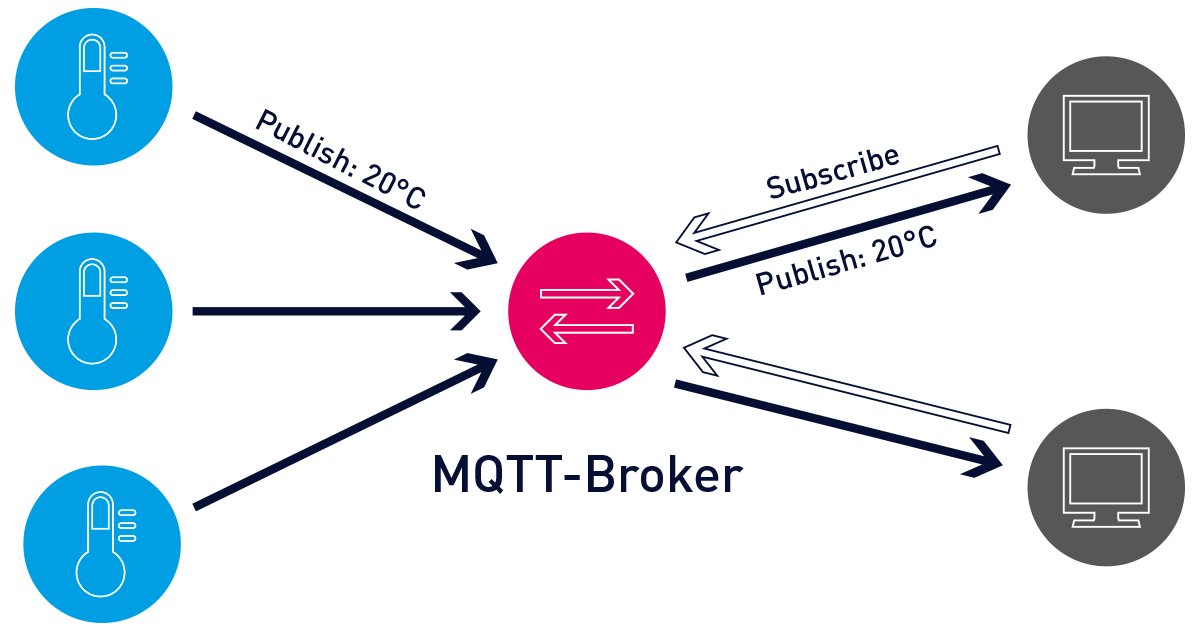
\includegraphics[width=0.7\linewidth]{images/chapter1-mqtt-architecture}
    \caption{Architettura Pub/Sub}
\end{figure}

%prima pagina
\section{L'architettura publisher/subscriber in MQTT}
\label{sec:mqtt-architettura}
Il modello architetturale publisher/subscriber si basa su tre componenti:
\begin{itemize}
    \item \textbf{Publisher}\newline
    Invia messaggi al broker.
    \item \textbf{Subscriber}\newline
    Richiede al broker di ricevere dei messaggi.
    \item \textbf{Broker}\newline
    Trasferisce i messaggi dai publisher ai subscriber.
\end{itemize}
I messaggi all'interno dell'architettura possono essere pubblicati in vari formati e possono essere filtrati in due modi:
in base al topic ("canale") oppure in base al contenuto.
Il filtro con topic prevede che i messaggi vengano categorizzati secondo dei canali.
Il publisher trasmette su un canale e il subscriber si deve iscrive a quel canale per ricevere solo quei messaggi.
Invece nel filtro con contenuto i messaggi non sono categorizzati.
I publisher inviano i messaggi e i subscriber definiscono un criterio con cui ricevere i messaggi. \newline
L'architettura permette il disaccoppiamento tra publisher e subscriber:
un publisher non conosce né gli altri publisher né i subscriber, e lo stesso vale per i subscriber.
Inoltre permette la comunicazione asincrona: il publisher non attende una risposta dopo l'invio.\newline
Nel caso specifico del protocollo MQTT, i messaggi sono organizzati secondo il filtro con topic
e vengono pubblicati in uno dei seguenti formati: JSON, XML, dati binari o testo.
I componenti assumono le seguenti denominazioni:
\begin{itemize}
    \item \textbf{Client publisher}\newline
    Pubblica sul broker messaggi su uno specifico topic.
    Questa operazione viene fatta da dispositivi come sensori.
    \item \textbf{Client subscriber}\newline
    Invia al broker la richiesta di iscrizione a uno o più topic.
    Questa operazione viene fatta da dispositivi che devono raccogliere o visualizzare i dati.
    \item \textbf{Broker MQTT}\newline
    È il sistema backend, chiamato impropriamente server, che coordina i diversi messaggi che arrivano dai client.
    Si può comparare a un ufficio postale che riceve i messaggi dai client "publisher" e li smista secondo un topic specifico.
    Successivamente li deve distribuire ai client "subscriber" iscritti a quel topic.
\end{itemize}
Un client in base alle funzioni che deve svolgere può essere publisher o subscriber oppure entrambi.


